%%This is a very basic article template.
%%There is just one section and two subsections.
\documentclass{article}

%definitions for Formelsammlung

\usepackage[left=1.5cm,right=1.5cm,top=2.5cm,bottom=2cm,landscape]{geometry} 
\usepackage{multicol}
\usepackage[ngerman]{babel}
\usepackage{tabularx}
\usepackage{mathpazo}
\usepackage{mathtools}
\usepackage{amsmath}  
\usepackage{setspace} 
\usepackage{commath}
\usepackage[utf8]{inputenc}
%\usepackage[ansinew]{inputenc}  
\usepackage[T1]{fontenc}
\usepackage{lmodern} 
\usepackage{hyperref}
\usepackage{bigints}
\usepackage{array}
\usepackage[table]{xcolor}
\usepackage{layouts}
\usepackage{siunitx}
\usepackage{wrapfig}
\usepackage{multirow,bigstrut}
\usepackage{trfsigns}
\usepackage{amssymb} 
\usepackage{fancyhdr}
\usepackage{datetime}
\usepackage{pgfplots}
\usepgfplotslibrary{fillbetween}
\usepackage{listings}
\usepackage{mathrsfs}
\usepackage{tabu}
\usepackage{pdflscape}
\usepackage{booktabs}
%\usepackage{mathabx}
\usepackage{graphicx}
\usepackage{supertabular}
\usepackage{siunitx}
\usepackage[europeanvoltages, europeancurrents, europeanresistors, americaninductors, smartlabels]{circuitikz}

\DeclareMathOperator\arctanh{arctanh}
\DeclareMathOperator\arsinh{arsinh} 
\DeclareMathOperator\arcosh{arcosh}
\DeclareMathOperator\artanh{artanh}
\DeclareMathOperator\arcoth{arcoth} 
\DeclareMathOperator\sinc{sinc} 
\DeclareMathOperator\sgn{sgn} 
\DeclareMathOperator\LPF{LPF} 
\DeclareMathOperator\Q{Q} 
\DeclareMathOperator\erf{erf} 
\DeclareMathOperator\var{Var} 
\DeclareMathOperator\Cov{Cov} 
\DeclareMathOperator\floor{floor} 
\DeclareMathOperator\E{E} 
\DeclareMathOperator\NDFT{DFT} 
\DeclareMathOperator\IDFT{IDFT} 


%colorCodes
\definecolor{listinggray}{gray}{0.9}
\definecolor{lbcolor}{rgb}{0.95,0.95,0.95}
\definecolor{lightGray}{gray}{0.1}

\definecolor{cOrange}{HTML}{996633}
\definecolor{clOrange}{HTML}{DBB48D}
\definecolor{cBlue}{HTML}{336699}
\definecolor{clBlue}{HTML}{A0BCD8}
\definecolor{cGreen}{HTML}{339966}
\definecolor{clGreen}{HTML}{94D4B4}
\definecolor{cRed}{HTML}{993333}
\definecolor{clRed}{HTML}{D0B0B0}
\definecolor{cGray}{gray}{0.4}
\definecolor{clGray}{gray}{0.96}



\setlength{\parindent}{0pt}
%\DeclareMathOperator\arctanh{arccot}
\newcolumntype{L}[1]{>{\raggedright\let\newline\\\arraybackslash\hspace{0pt}}m{#1}}
\newcolumntype{C}[1]{>{\centering\let\newline\\\arraybackslash\hspace{0pt}}m{#1}}
\newcolumntype{R}[1]{>{\raggedleft\let\newline\\\arraybackslash\hspace{0pt}}m{#1}}
\newcolumntype{Y}{>{\centering\arraybackslash}X}
\newcolumntype{Z}{>{\raggedleft\arraybackslash}X}
\newcommand{\fmm}{\displaystyle} 
\newcommand{\cn}[1]{\underline{#1}} 
\newcommand{\hlaplace}{\quad\laplace\quad}
\newcommand{\hLaplace}{\quad\Laplace\quad}
\newcommand{\ztransform}{\, \, \xrightarrow{\, \, z\, \, } \, \,}
\newcommand{\zTransform}{\, \, \xrightarrow{\, \, z^{-1}\, \, } \, \, }
\newcommand{\infint}{\int_{-\infty}^{+\infty}}
\newcommand{\infiint}{\iint_{-\infty}^{+\infty}}
\newcommand{\limint}{\lim_{T\rightarrow \infty} \frac{1}{T} \int_{-T/2}^{T/2}}
\newcommand{\bedeq}{\mathrel{\stackrel{\makebox[0pt]{\mbox{\normalfont\tiny WSS}}}{=\joinrel=}}}
\renewcommand{\fourier}{\mathcal{F}}
\newcommand{\infsum}[1]{\sum_{#1 = -\infty}^{\infty} }
\newcommand{\cif}{\text{if}\:}
\newcommand{\cand}{\:\text{and}\:}
\newcommand{\celse}{\text{otherwise}\:}
\renewcommand{\abs}[1]{\left| #1 \right|}
\newcommand{\cvec}[1]{\left[\begin{smallmatrix} #1 \end{smallmatrix}\right]}
\newcommand{\vvec}[1]{\renewcommand*{\arraystretch}{0.8}\left[\begin{array}{c} #1 \end{array}\right]}
\renewcommand{\hat}[1]{\widehat{#1}}
\let\oldsi\si
\renewcommand{\si}[1]{\; \left[\oldsi[per-mode = fraction]{#1}\right]}

\newcommand{\plotTF}[1]{
\begin{tikzpicture}
\begin{axis}[xlabel=$\omega$,ylabel=$\abs{H(\omega}$, xmin = 0, xmax = 3.5, ymin = 0, ymax = 1, xtick = {3.14}, xticklabel={$\pi$}, ytick={0}, axis lines=middle, width=6cm, height=4cm, 
every axis x label/.style={at={(ticklabel* cs:1.05)},anchor=west}]
\addplot[name path=H, domain=0:3.14, samples=200] {#1};
\path[name path=axis] (axis cs:0,0.01) -- (axis cs:3.14,0.01);
\addplot[fill=clGray] fill between[of=H and axis, soft clip={domain=0.01:3.14}];
\end{axis}
\end{tikzpicture}
}

\newenvironment{donotbrake}{\begin{minipage}{\columnwidth}}{
\end{minipage} \vspace{1em}}

\newenvironment{cmat}[1]{
  \renewcommand*{\arraystretch}{0.9}
  \left[
  \begin{array}{#1}
}{
  \end{array}
  \right]
}

\newenvironment{case}{
  \left\{ \begin{array}{ll}
}{
  \end{array} \right.
}


\newenvironment{scase}{
  \renewcommand*{\arraystretch}{1}
  \left\{ \begin{array}{ll}
  }{
  \end{array} \right.
}

\newcommand\xdownarrow[1][2ex]{%
   \mathrel{\rotatebox{90}{$\xleftarrow{\rule{#1}{0pt}}$}}
}

\newcommand{\ncr}[2]{\binom{#1}{#2}}

\renewenvironment{description}{\color{cGray}}{}
\newenvironment{definition}{\color{cGray}}{} 
\newcommand{\cdef}[1]{\begin{definition}#1\end{definition}}


\newcommand{\vLaplace}[1][]{\mbox{\setlength{\unitlength}{0.1em}%
        \begin{picture}(10,20)%
          \put(3,2){\circle{4}}%
          \put(3,4){\line(0,1){12}}%
          \put(3,18){\circle*{4}}%
          \put(10,7){#1}
        \end{picture}%
       }%
 }%

\newcommand{\vlaplace}[1][]{\mbox{\setlength{\unitlength}{0.1em}%
        \begin{picture}(10,20)%
          \put(3,2){\circle*{4}}%
          \put(3,4){\line(0,1){12}}%
          \put(3,18){\circle{4}}%
          \put(10,7){#1}
        \end{picture}%
       }%
 }%         
 
           
\newenvironment{blockdiagram}[1]{
	\begin{tikzpicture}
		[auto, node distance=2.5cm,>=latex', scale=#1, every node/.style={scale=#1}]
}{
	\end{tikzpicture}
} 
 
 
\renewcommand{\arraystretch}{1.5}


\newenvironment{mtabular}[1] {
  \renewcommand{\arraystretch}{2}
  
  \begin{tabular}{#1}
}  
{
  \end{tabular}
  
  \renewcommand{\arraystretch}{1.5}
}

\newenvironment{lmtabular}[1] {
\renewcommand{\arraystretch}{2}

\begin{supertabular}{#1}
}  
{
\end{supertabular}

\renewcommand{\arraystretch}{1.5}
}

\newenvironment{dtabular} {
  \begin{tabular}{>{\begin{definition}}l<{\end{definition}} >{\begin{definition}}l<{\end{definition}}}
}  
{
  \end{tabular}
}

\newenvironment{ddtabular} {
  \begin{center}
  \begin{tabular}{>{\begin{definition}}l<{\end{definition}} >{\begin{definition}}l<{\end{definition}} | >{\begin{definition}}l<{\end{definition}} >{\begin{definition}}l<{\end{definition}}}
}  
{
  \end{tabular}
  \end{center}
}


%configure tikz
%system description
\usetikzlibrary{shapes,arrows}
\usetikzlibrary{decorations.markings}
\usetikzlibrary{calc}
\tikzstyle{block} = [draw, rectangle, minimum height=2.5em, minimum width=5em]
\tikzstyle{input} = [coordinate]
\tikzstyle{output} = [coordinate]
\tikzstyle{pinstyle} = [pin edge={to-,thin,black}]
\tikzstyle{sum} = [draw, circle, node distance=1em, minimum height=1.5em]
\tikzset{
	>=latex,
	photon/.style={decorate,decoration={snake,post length=1mm, segment length = 2mm, amplitude=0.6mm}}
}
\tikzset{->-/.style={decoration={
			markings,
			mark=at position #1 with {\arrow{>}}},postaction={decorate}}}
\tikzset{%
  block/.style    = {draw, thick, rectangle, minimum height = 2.5em,
    minimum width = 3em},
  sum/.style      = {draw, circle, node distance = 1.5cm}, % Adder
  input/.style    = {coordinate}, % Input
  output/.style   = {coordinate}, % Output
  gain/.style     = {draw, thick, isosceles triangle, minimum height = 2em, isosceles triangle apex angle=60},
  rgain/.style    = {draw, thick, isosceles triangle, minimum height = 2em, isosceles triangle apex angle=60}
}


%externalize TIKZ
%\usetikzlibrary{external}
%\tikzexternalize[prefix=tikz/]

%lstlisting

\lstset{
  backgroundcolor=\color{lbcolor},
  tabsize=2,    
% rulecolor=,
  language=[GNU]C++,
  basicstyle=\scriptsize,
  upquote=true,
  aboveskip={1.5\baselineskip},
  columns=fixed,
  showstringspaces=false,
  extendedchars=false,
  breaklines=true,
  prebreak = \raisebox{0ex}[0ex][0ex]{\ensuremath{\hookleftarrow}},
  frame=single,
  numbers=none,
  showtabs=false,
  showspaces=false,
  showstringspaces=false,
  identifierstyle=\ttfamily,
  keywordstyle=\color{cBlue}
  commentstyle=\color{cGreen},
  stringstyle=\color{cRed},
  numberstyle=\color{black},
% \lstdefinestyle{C++}{language=C++,style=numbers}’.
}
\lstset{
  backgroundcolor=\color{lbcolor},
  tabsize=2,
  language=C++,
  captionpos=b,
  tabsize=3,
  frame=lines,
  numbers=none,
  numberstyle=\tiny,
  numbersep=5pt,
  breaklines=true,
  showstringspaces=false,
  basicstyle=\ttfamily,
  identifierstyle=\color{cOrange},
  keywordstyle=\color{cBlue},
  commentstyle=\color{cGreen},
  stringstyle=\color{cRed}
}

\lstdefinelanguage{makefile}{
  morekeywords={cc,CFLAGS,LFLAGS,OBJ,EXE},
  morecomment=[l]{\#}
}

\lstdefinestyle{makefile}{
  language=makefile,
  basicstyle=\ttfamily,
  keywordstyle=\color{cBlue},
  commentstyle=\color{cGreen},
  frame=lines,
  numbers=none,
  backgroundcolor=\color{lbcolor}
}


\newcolumntype{M}{>{$}c<{$}} % math-mode version of "c" column type

%header & footer
\pagestyle{fancy}
\lhead{Tibor Schneider}
\rhead{Seite \thepage}
\cfoot{\today} 

\renewcommand{\headrulewidth}{0.4pt}
\renewcommand{\footrulewidth}{0.4pt}

%Title of Document
\chead{Physics II - Summary} 

\begin{document}
\begin{twocolumn} 



\section{The Photon}  

\begin{donotbrake}
\begin{tabular}{cc}
	\begin{dtabular}
		
		$c \si{\metre \per \second}$ & speed of light \\
		$h \si{\metre \squared \kilogram \per \second}$ & planc's constant \\
		$e \si{\coulomb}$ & electorn charge \\
		$m_e \si{\kilogram}$ & electron mass \\
		$k_B \si{\metre \squared \kilogram \per \second \squared \per \kelvin}$ & bolzmann constant \\
		$\epsilon_0 \si{\farad \per \metre}$ & vacuum permittivity \\
		
	\end{dtabular}

	\begin{mtabular}{c}
		$c = 2.998 \cdot 10^8 \si{\metre \per \second}$ \\
		$h = 6.626 \cdot 10^{-34} \si{\metre \squared \kilogram \per \second}$ \\
		$\hslash = \frac{h}{2\pi}$ \\
		$e = 1.602 \cdot 10^{-19} \si{\coulomb}$ \\
		$m_e = 9.109 \cdot 10^{-31} \si{\kilogram}$ \\
		$k_B = 1.381 \cdot 10^{-23} \si{\metre \squared \kilogram \per \second \squared \per \kelvin}$ \\
		$\epsilon_0 = 8.854 \cdot 10^{-12} \si{\farad \per \meter}$ \\
		$1 \si{\electronvolt} = 1.602 \cdot 10^{-19} \si{\joule}$ \\
	\end{mtabular}
\end{tabular}
\end{donotbrake}

\begin{donotbrake}
\subsection{Photon \& Electron}

\begin{tabular}{cc}
	\begin{dtabular}
		$\lambda \si{\meter}, \, \nu\si{\per\second}$ & Wavelength, Freq. \\
		$k$ & Wavenumber \\
		$E \si{\joule}$ & Energy \\
		$\vec{F_c} \si{\newton}$ & Coulomb Force \\
	\end{dtabular} &
	\begin{mtabular}{c}
		$\fmm \lambda = \frac{c}{\nu} \quad \fmm \nu = \frac{c}{\lambda} \quad \omega = 2 \pi \nu$ \\
		$\fmm k = \frac{2 \pi \nu}{c}$ \\
		$E = h \cdot \nu = \hslash \cdot \omega$ \\
		$\fmm \abs{\vec{F_c}} = \frac{Q_1 \cdot Q_2}{4 \pi \epsilon_0 r^2}$ \\
	\end{mtabular}
\end{tabular}

\end{donotbrake}


\begin{donotbrake}
\subsection{Photoelectric effect}

\begin{tabular}{cc}
	\begin{dtabular}
		$V \si{\volt}$ & Voltage \\
		$\phi_0 \si{\electronvolt} $ & Work function \\
		$I \si{\ampere}$ & Photo-current \\
		$n \si{\metre^{-3}}$ & Volume density of electrons \\
		$A \si{\metre \squared}$ & Area \\
		$v \si{\metre \per \second}$ & velocity of electrons \\	
	\end{dtabular} &
	\begin{mtabular}{c}
		$\fmm h \nu - \phi_0 = \frac{1}{2} m v^2 = eV$ \\
		$\fmm V(\nu) =  \frac{h}{e} \nu - \frac{\phi_0}{e}$ \\
		$\fmm I = n A v e$ \\
	\end{mtabular}
\end{tabular}
\end{donotbrake}


\begin{donotbrake}
\subsection{Blackbody Radiation}

\begin{ddtabular}
	$L \si{\metre}$ & length of blackbody cube &
	$k_i$ & wave constants \\
	$E_x$ & Electric field in x-direction &
	$<E>$ & Average Energy \\
	$N$ & Number of states &
	$D$ & Density of states \\
	$u$ & Blackbody radiation &
	$I$ & Power radiated \\
\end{ddtabular}

\begin{mtabular}{c}
	$E_x(x,y,z) = E_{0x} \cos(k_x x) sin(k_y y) sin(k_z z)$ \\
	$\fmm k_x = n \frac{\pi}{L} \quad \fmm k_y = m \frac{\pi}{L} \quad \fmm k_z = l \frac{\pi}{L} \qquad k = \sqrt{k_x^2 + k_y^2 + k_z^2}$ \\
	$\fmm N(k) = \frac{1}{3\pi^2} k^3 L^3 \qquad D(k) = \frac{k^2}{\pi^2}$ \\
	$\fmm u(\omega) =\frac{\omega^2}{\pi^2 c^3} \cdot \frac{\hslash \omega}{\exp\left(\frac{-\hslash \omega}{k T}\right)-1} d\omega \qquad u(\nu) = \frac{8\pi h \nu^3}{c^3 \left( \exp \left(\frac{h \nu}{k T}\right) - 1\right)} d\nu$ \\
	$\fmm I(\omega) = c \cdot u(\omega)$
\end{mtabular}

\textbf{Equipartition-Theorem}: Each degree of Freedom has an energy of $kT$
\end{donotbrake}

\begin{donotbrake}
\subsection{Johnson-Noise}

This is the noise created in a one-dimensional circuit (like a coax-cable).

\begin{tabular}{cc}
	
	\begin{tabular}{c}
	  \begin{circuitikz} [scale=0.7, transform shape]
	  	\draw [thick] (1,2) to [short] (5,2);
	  	\draw [thick] (1,0) to [short] (5,0);
	  	\draw (1,0) to [short, o-] (0,0) to [R=$R$] (0,2) to [short, -o ](1,2);
	  	\draw (5,0) to [short, o-] (6,0) to [R=$R$] (6,2) to [short, -o ](5,2);
	  	\draw (3,1.2) node {$Z_c = R$};
	  	\draw [latex-latex] (1,0.3) -- (5,0.3) node [pos=0.5, above] {$L$};
  	\end{circuitikz} \\ $\qquad$
	  \begin{circuitikz} [scale=0.7, transform shape]
	  	\draw (0,0) to [R=$R'$] (0,2) to [sV_=$V$] (4,2) to [R=$R$] (4,0) to [short] (0,0);
	  	\draw [dashed] (-0.8,-0.6) rectangle (2.6,2.6);
	  \end{circuitikz}
	\end{tabular} &

	\begin{tabular}{c}
		\begin{dtabular}
			$\langle V^2\rangle$ & Noise Voltage \\
			$\Delta \nu$ & Bandwidth \\
		\end{dtabular} \\
		\begin{mtabular}{c}
			$E = E_0 \cdot \sin(k_x \cdot x)$ \\
			$\langle V^2 \rangle = 4 R \cdot k_BT \cdot \Delta \nu$
		\end{mtabular}
	\end{tabular}
\end{tabular}
\end{donotbrake}

\begin{donotbrake}
\subsection{Momentum of a photon}

\begin{tabular}{cc}
	\begin{tabular}{c}
		\begin{tikzpicture}
			\draw (2,0) rectangle (2.2,3);
			\draw [->, photon] (0,0.5) -- (2,1.5);
			\draw [->, photon] (1.9,1.6) -- (0,2.5);
			\draw [->] (2.2,1.5) -- (3,1.5) node[pos=0.5, above] {$v$};
		\end{tikzpicture}
	\end{tabular} &
	\begin{tabular}{c}
		\begin{dtabular}
			$p  \si{\kilo \gram \metre \per \second}$ &momentum \\
		\end{dtabular} \\
		\begin{mtabular}{c}
			$\fmm p_{absorbing} =\frac{h \nu}{c}=m\cdot v$ \\
			$\fmm p_{reflecting} =2 \cdot \frac{h \nu}{c}$
		\end{mtabular}
	\end{tabular}
\end{tabular}
\end{donotbrake}

\begin{donotbrake}
\subsection{Absorption, spontaneous and stimulated emission}
\begin{center}
\begin{tabular}{ccc}
	\begin{tikzpicture}
		\draw[thick] (0,0) -- (1,0) (0,2) -- (1,2);
		\draw[*->] (0.5,0) -- (0.5,2) node[pos=0.5, right]{$B_{12}$};
		\draw[->,photon] (-0.5,1) -- (0.5,1);
	\end{tikzpicture} &
	\begin{tikzpicture}
	\draw[thick] (0,0) -- (1,0) (0,2) -- (1,2);
	\draw[<-*] (0.5,0) -- (0.5,2) node[pos=0.5, left]{$A_{21}$};
	\draw[->,photon] (0.5,1) -- (1.5,1);
	\end{tikzpicture} &
	\begin{tikzpicture}
	\draw[thick] (0,0) -- (1,0) (0,2) -- (1,2);
	\draw[<-*] (0.5,0) -- (0.5,2) node[pos=0.8, right]{$B_{21}$};
	\draw[->,photon] (-0.5,1) -- (0.5,1);
	\draw[->,photon] (0.5,1.2) -- (1.5,1.2);
	\draw[->,photon] (0.5,0.8) -- (1.5,0.8);
	\end{tikzpicture} \\
	absorbtion & spontaneous emission & stimulated emission
\end{tabular}
\end{center}

\begin{center}
	\begin{dtabular}
		$n_1$ & Number of electrons in the lower energy state \\
		$n_2$ & Number of electrons in the higher energy state \\
	\end{dtabular} 
\end{center}

$$\fmm \frac{dn_2}{dt} = \underbrace{n_1 \cdot u(\nu) \cdot B_{12}}_\text{absorbtion} - \underbrace{n_2 \cdot u(\nu) \cdot B_{21}}_\text{stimulated emission} - \underbrace{n_2 \cdot A_{21}}_\text{spontaneous emission} $$
$$\fmm \frac{n_2}{n_1} = e^{-\frac{h \nu}{k_B T}} = \frac{u(\nu) B_{12}}{u(\nu) B_{21} + A_{21}}$$
$$\fmm B_{21} = B_{12} = B \qquad A_{21} = \frac{8\pi h \nu^3}{c^3}$$

\end{donotbrake}

\begin{donotbrake}
\subsection{Laser-optical amplification}

\begin{center}
	\begin{tabular}{cc}
		\begin{tikzpicture}
		\draw [-implies, double equal sign distance] (0.3,0.5) -- (0.3,3.5) node[pos=0.5, left] {R};
		\draw [->, dashed] (0.7,3.5) -- (1.5,3);
		\draw [->, dashed] (1.5,1) -- (0.7,0.5);
		\draw [->] (1.5,3) -- (1.5,1);
		\draw [thick] (0,0.5) -- (1,0.5) node[right]{0} (0,3.5) -- (1,3.5) node[right] {3} (1,3) -- (2,3) node[right] {2} (1,1) -- (2,1) node[right] {1};
		\end{tikzpicture} &
		\begin{tikzpicture}
		\draw [fill=black!5] (1,0) -- (1,2) -- (5,2) node[pos=0.5, above] {amplification medium} -- (5,0) -- (1,0);
		\draw [thick] (0,0) arc (-150:-210:2);
		\draw [thick] (6,0) arc (-30:30:2);
		\draw [->-=.35] (-0.1,1.8) arc ( 250: 290:9.05);
		\draw [->-=.75] (-0.1,1.8) arc ( 250: 290:9.05);
		\draw [->-=.75] ( 6.1,1.8) arc ( -70: -110:9.05);
		\draw [->-=.35] ( 6.1,1.8) arc ( -70: -110:9.05);
		\draw [->-=.35] (-0.1,0.2) arc (-250:-290:9.05);
		\draw [->-=.75] (-0.1,0.2) arc (-250:-290:9.05);
		\draw [->-=.75] ( 6.1,0.2) arc (70:110:9.05);
		\draw [->-=.35] ( 6.1,0.2) arc (70:110:9.05);
		\draw [implies-,double equal sign distance] (3,0) -- (3,-0.5) node[below] {pump};
		\draw [->, dashed] (6.3,1) -- (7.3,1);
		\draw [->, dashed] (6.2,1.5) -- (7.3,1.5);
		\draw [->, dashed] (6.2,0.5) -- (7.3,0.5);
		\draw (6,2) node[above] {cavity};
		\end{tikzpicture}
	\end{tabular}
\end{center}

Electrons are excited from the ground state ``0'' to the level ``3'' by pumping through incoherent radiation. 
The electrons then fall onto a long-lived state $n_2$ (State ``2'') from level ``3''. 
The pumping can be done either optically by shining a strong incoherent light or by passing a current. 
It is also assumed that the lower state is quickly emptied by a fast process with lifetime $\tau_1$. 
As a result, the population in state ``2'' is:
$$n_2 = \frac{R}{A_{21}} \quad \text{whereas} \quad n_1 \approx 0 \quad \text{because} \quad  A_{21} < \frac{1}{\tau_1}$$
We have rherefore a population inversion between the two states. 
The likelihood of a stimulated emission process is larger than the one of absorbtion. 
If we enclose the system in an optical cavity, we can achieve self-sustained oscillation at the frequency $\nu$.

\end{donotbrake}

\section{Wave mechanics}

\begin{center}
	\begin{tabular}{ccccc}
		& frequency & wavelength & momentum & energy \\
		\midrule
		Particle & & $\lambda_b = \frac{h}{p}$ & $p = m v$ & $E = \frac{1}{2} m v^2$ \\
		Wave & $\omega$ & $\lambda = \frac{2\pi c}{\omega}$ & $p = \frac{\hslash \omega}{c}$ & $E = \hslash \omega$ \\
	\end{tabular}
\end{center}

\begin{donotbrake}
\subsection{Compton Scattering}

\begin{tabular}{cc}
	\begin{tabular}{c}
		\begin{tikzpicture}
			\draw [->, photon] (0,0) -- (1.3,0) node[pos=0.5, below] {$p_1$};
			\draw [fill=black] (2,-0.1) circle (0.08) node[below] {$e^-$};
			\draw [->, photon] (4,0) -- (5.5,1) node[pos=0.5, above left]{$p_2$};
			\draw [fill=black] (4,0) circle (0.08) node[below] {$e^-$};
			\draw [->] (4,0) -- (5.5,-1.3) node[pos=0.7, below] {$v$};
			\draw [dashed] (4,0) -- (5.5,0);
			\draw (4.8,0) arc (0:33:0.8) node[pos=0.6, right] {$\theta$};
			\draw (4.9,0) arc (0:-41:0.9) node[pos=0.6, right] {$\phi$};
		\end{tikzpicture}
	\end{tabular} &
	\begin{mtabular}{c}
		$\fmm p_1 =\frac{h \nu_1}{c} \qquad p' = \frac{h \nu_2}{c}$ \\
		$\fmm \nu_2 = \nu_1 - \frac{P_e^2}{2 m_e h}$ \\
		$\fmm \lambda_2 - \lambda_1 = \frac{h}{m_e c} (1 - \cos \theta)$;
	\end{mtabular}
\end{tabular}
\end{donotbrake}


\begin{donotbrake}
	\subsection{Double Slit and Bragg Diffraction}
	
	\begin{tabular}{ccc}
		\begin{tabular}{c}
			\begin{tikzpicture} [scale=0.8, transform shape]
			\draw [fill=black!10] (-0.05,0.05) rectangle (0.05,0.85) (-0.05,0.95) rectangle (0.05,1.45) (-0.05,1.55) rectangle (0.05,2.35);
			\draw [|-|] (-0.2,1.5) -- (-0.2,0.9) node [pos=0.5,left] {\small $a$};
			\draw [dashed] (0,1.2) -- (2,1.2);
			\draw (0,1.2) -- (2,0.6);
			\draw (1.5,1.2) arc (0:-17:1.5);
			\draw (1.2,1) node {\small $\theta$}; 
			\end{tikzpicture}
		\end{tabular} &
		
		\begin{tabular}{c}
			\begin{tikzpicture} [scale=0.8, transform shape]
			\foreach \y in {0,0.4,0.8,1.2,1.6,2.0} {
				\draw [fill=black!10] (-0.05,\y+0.05) rectangle (0.05,\y+0.35);
			}
			\draw [|-|] (0.2,0.8) -- (0.2,0.4) node[pos=0.5, right] {\small $a$};
			\draw [dashed] (0,1.6) -- (2,1.6);
			\draw (0,1.6) -- (2,1);
			\draw (1.5,1.6) arc (0:-17:1.5);
			\draw (1.2,1.4) node {\small $\theta$}; 
			\end{tikzpicture}
		\end{tabular} &
		\begin{mtabular}{cl}
			Constructive & $\fmm \sin \theta = \frac{n \lambda}{a}$ \\
			Destructive &$\fmm \sin \theta = \frac{(n +\frac{1}{2}) \lambda}{a} $ \\
			 & $n \in \mathbb{Z}$
		\end{mtabular}
	\end{tabular}
\end{donotbrake}

\begin{donotbrake}
\subsection{Single slit}

\begin{tabular}{cc}
	\begin{tabular}{c}
		\begin{tikzpicture}[scale=0.7, transform shape]
			\draw [->, photon] (-1.5,1) -- (-0.7,1);
			\draw [thick] (0,-0.5) -- (0,0.7) -- (0.1,0.7) -- (0.1,-0.5);
			\draw [draw=none, fill=black!10] (0,-0.5) rectangle (0.1,0.7); 
			\draw [thick] (0,2.5) -- (0,1.3) -- (0.1,1.3) -- (0.1,2.5);
			\draw [draw=none, fill=black!10] (0,2.5) rectangle (0.1,1.3);
			\draw [|-|] (-0.2,0.7) -- (-0.2,1.3) node[pos=0.5, left] {$a$};
			\draw (2,-0.5) -- (2,2.5);
			\draw [thick, domain=-1.51:1.5, samples=150, variable=\y] plot ({30*sin(\y*200)*sin(\y*200)/((\y*20)*(\y*20)) + 2},{\y + 1}); 
			\draw (2.5,1.8) node {$I(\theta)$};
			\draw [dashed] (0,1) -- (2,1);
			\draw (0,1) -- (1.95,1.75);
			\draw (1.5,1) arc (0:21:1.5) node[pos=0.5, left] {$\theta$};
		\end{tikzpicture}
	\end{tabular} &
	\begin{mtabular}{c}
		$\fmm I(\theta) = I_0 \frac{\sin^2 \theta}{\theta^2}$ \\
		$\fmm \sin \theta = \frac{\lambda}{a}$
	\end{mtabular}
\end{tabular}
\end{donotbrake}

\subsection{Bohr-Sommerfeld equalization}

Every single particle must satisfy the following equation. The quantized energy levels below relate to the hydrogen atom

\begin{tabular}{cc}
	\begin{dtabular}
		$p$ & Momentum of particle \\
		$E_n$ & Energy of the nth state \\
		$E_{ry}$ & Rydberg Energy \\
		$a_0$ & Bohr-radius \\
		$Z$ & Number of protons \\	
	\end{dtabular} &
	\begin{mtabular}{c}
		$\fmm \int_{length} p \cdot ds = n \cdot h \qquad n \in \mathbb{N}$ \\
		$\fmm E_n = -\frac{Z}{n^2} \cdot \frac{m_e e^4}{8 \epsilon_0^2 h^2} = - \frac{Z}{n^2} \cdot E_{ry} $ \\
		$\fmm r_n = \frac{n^2}{Z} \cdot \frac{2 \epsilon_0 h}{m_e e^2} = \frac{n^2}{Z} \cdot a_0$ \\
		$E_{ry} = 13.6 \si{\electronvolt}$ \\
		$a_0 = 5.292 \cdot 10^{-11} \si{\meter}$
	\end{mtabular}
\end{tabular}

\section{Quantum Mechanics}

\begin{donotbrake}
\subsection{Wave function}
$$\psi(\bm{x}, t): \mathbb{R}^4 \rightarrow \mathbb{C} \qquad \iiint \abs{\psi(\bm{x},t)}^2 d^3r = 1 $$
$$\psi(\bm{x}, t) = a \psi_1(\bm{x},t) + b \psi_2(\bm{x}, t), \qquad \abs{a}^2 + \abs{b}^2 = 1$$
\end{donotbrake}

\begin{donotbrake}
\subsection{The Schrödinger equation}

\begin{ddtabular}
	$V(x,t)$ & potential &
	$m$ & mass \\
\end{ddtabular}

$$i \hslash \cdot \frac{\partial \psi}{\partial t}(\bm{x},t) = - \frac{\hslash^2}{2m} \cdot \nabla^2 \psi(\bm{x},t) + V(\bm{x}, t) \psi(\bm{x},t)$$
$$\nabla^2 = \frac{\partial^2}{\partial x^2} + \frac{\partial^2}{\partial y^2} + \frac{\partial^2}{\partial z^2}$$
$$\psi = A \cdot e^{i (\bm{k} \bm{x} - \omega t)} \qquad \bm{k} = \Vector[&]{k_x,k_y,k_z}, \quad \bm{x} =\Vector{x,y,z}$$
$$E = \omega \hslash = \frac{\hslash^2 k^2}{2 m}, \qquad k^2 = \abs{k}^2$$

\end{donotbrake}

\begin{donotbrake}
\subsubsection{Phase and Group Velocity}

The \cdef{phase velocity $v_{\varphi}$} describes how fast the phase of the wave moves forward. 
The \cdef{group velocity $v_g$} describes how fast the energy is moving forward. 
$$v_{\varphi} = \frac{\omega}{k} \qquad v_g =\frac{\partial \omega}{\partial k}$$
For a particle wave, the phase velocity $v_{\varphi}$ is half the group velocity $v_g$
$$v_{\varphi} \cdot 2 = v_g$$
\end{donotbrake}

\begin{donotbrake}
\subsubsection{Stationary (Time independent) States}

In a stationary state, the wave function is a product of a function $\varphi(\bm{x})$ independent of time and a function $\chi(t)$ independent of space. 

$$\psi_n(\bm{x},t) = \varphi_n(\bm{x}) \cdot \chi_n(t) = \varphi_n(\bm{x}) \cdot e^{-i \frac{E_n}{\hslash}t}$$
$$-\frac{\hslash^3}{2m} \nabla^2 \varphi_n(\bm{x}) + V(\bm{x}) \varphi_n(\bm{x}) =\varphi_n(\bm{x}) \cdot E_n$$
$$\iiint \abs{\psi}^2 d^3\bm{x} = \iiint \abs{\varphi}^2 d^3\bm{x} = 1$$
$$\psi(\bm{x},t) = \sum a_n \varphi_n(\bm{x}) \cdot e^{-i \frac{E_n}{\hslash}t} \quad \sum \abs{a_n}^2 = 1$$

Requirements: The wave function must be continous, as well as it's derivative 
\end{donotbrake}

\subsubsection{Example: 1D infinite potential well}

\begin{tabular}{cc}
	\begin{tabular}{l}
		\begin{tikzpicture}
			\draw [fill=black!10, draw=none] (0,0) rectangle (1,2) (3,0) rectangle(4,2);
			\draw [->] (0,0) -- (4.1,0) node[right] {$x$};
			\draw [->] (1,0) -- (1,2.1) node[below right] {$V(x)$};
			\draw (3,0) -- (3,2);
			\draw (0.5,1) node {1} (2,1) node {2} (3.5,1) node {3};
			\draw (1,0) node[below] {0} (3,0) node[below] {$L$};
		\end{tikzpicture}
	\end{tabular} &
  \begin{mtabular}{l}
  	$\fmm \psi_{1} =\psi_{3} = 0$ \\
  	$\fmm -\frac{\hslash^3}{2m} \frac{\partial^2}{\partial x^2} \varphi_2(x,t) = E \varphi_2(x,t)$ \\
  	$\fmm \varphi_2 = A \sin(k x) + B \cos(k x)$ \\
  	Boundary cond.: $\fmm \varphi_2(0) = \varphi_2(L) = 0$ \\
  \end{mtabular}
\end{tabular}

\begin{mtabular}{c}
	$\fmm \varphi_{2_n} = A \cdot \sin (k_n x) \quad \psi_{2_n} = A \cdot \sin \left( k_n x \right)  \cdot e^{-i \frac{E_n}{\hslash} x}, \quad \text{\small Normalize:} \quad  A = \sqrt{\frac{2}{L}}$ \\
	$\fmm E_n =n^2 \cdot \frac{\hslash^2 \pi^2}{2 m L} =n^2 \cdot E_0, \qquad k_n = \frac{n \pi}{L}$ \\
\end{mtabular}

\subsubsection{Example: 1D finite potential well}

\begin{tabular}{cc}
	\begin{tabular}{l}
		\begin{tikzpicture}
			\draw [->] (0,1.5) -- (4,1.5) node[right] {$x$};
			\draw [->] (2,0) -- (2,2) node[above] {$V(x)$};
			\draw [thick] (0,1.5) -- (1,1.5) -- (1,0.25) -- (3,0.25) -- (3,1.5) -- (3.9,1.5);
			\draw (0.5,1) node {1} (2,1) node[right] {2} (3.5,1) node {3};
			\draw (1,1.5) node[above] {$-L$} (3,1.5) node[above] {$L$};
			\draw (2,0.25) node[above left] {$-V_0$};
		\end{tikzpicture}
	\end{tabular} &
	\begin{tabular}{p{0.5\columnwidth}}
		The Energy $E$ can be either bigger or smaller than 0. If $E>0$, the wave function will decay exponentially in region 1 and 3. If $E < 0$, the wave will propagate away from the potential well.
	\end{tabular}
\end{tabular}

\begin{donotbrake}
\textbf{Inside the well: }The general solution to the rearranged Schrödinger's is:

$$-\frac{\hslash^2}{2m} \frac{\partial^2}{\partial x^2}\varphi_2(x) = (E-V_0) \varphi_2(x)$$
$$\varphi_2(x) = A_2 e^{i k x} + A'_2 e^{-i k x} \qquad E = \frac{k^2 \hslash^2}{2m} \quad k = \sqrt{\frac{2 m (E-V_0)}{\hslash^2}}$$

\end{donotbrake}

\begin{donotbrake}

\textbf{Outside the well: }There are two cases, which can apply:

$$-\frac{\hslash}{2m} \frac{\partial^2}{\partial x^2}\varphi_{1}(x) = E \varphi_{1}(x)$$

\begin{enumerate}
	\item $E > 0$:\textbf{Unbound state}
	$$ \varphi_1 =  A_1 e^{i k x} + A'_1 e^{-i k x} \qquad k = \sqrt{\frac{2 m E}{\hslash^2}}$$
	The unbound state does not make sense to be investigated, because the particle is free to be anywhere. In the following, only the unbound state is considered.
	\item $E < 0$: \textbf{Bound state}
	$$\varphi_1 = B_1 e^{\delta x} + B'_1 e^{-\delta x} \qquad \delta = \sqrt{-\frac{2 m E}{\hslash^2}}$$
	
	We see that as $x \rightarrow -\infty$, the Term $B'_1$, as well as $B_3$ approaches $\infty$. Since the wave function cannot approach $\infty$, $B'_1 = B_3 = 0$ is a condition.
	
	$$\varphi = \begin{case}
		\varphi_1 = B_1 e^{\delta x} & x < -L \\
		\varphi_2 = A_2 e^{i k x} + A'_2 e^{-i k x} & -L < x < L \\
		\varphi_3 = B'_3 e^{-\delta x} & L < x
		
	\end{case}$$
	  
\end{enumerate}
\end{donotbrake}

\begin{donotbrake}
	
\textbf{Boundary conditions:} We require, that the wave function is continuous, as well as it's spacial derivative. Therefore, we have:

$$\varphi_1 (-L) =\varphi_2(-L) \qquad \varphi_2 (L) = \varphi_3(L)$$
$$\frac{\partial}{\partial x}\varphi_1 (-L) = \frac{\partial}{\partial x}\varphi_2(-L) \qquad \frac{\partial}{\partial x}\varphi_2 (L) =\frac{\partial}{\partial x}\varphi_3(L)$$

\end{donotbrake}

\begin{mtabular}{C{0.45\columnwidth}|C{0.45\columnwidth}}
	\textbf{Even solutions}: only even (cosine) components &
	\textbf{Odd solutions}: only odd (sine) components \\
	$\fmm \abs{\cos \left(k L\right)} =\frac{k}{k_o}, \quad \tan (k L) > 0$ &
	$\fmm \abs{\sin \left(k L\right)} =\frac{k}{k_o}, \quad \tan (k L) > 0$ \\
	$\fmm k_0 = \sqrt{\frac{2 m V_0}{\hslash^2}}$ & 
	$\fmm k_0 = \sqrt{\frac{2 m V_0}{\hslash^2}}$ \\
	
	\begin{tikzpicture}
	\begin{axis}[xlabel=$k$,ylabel=$\abs{\cos(kL)}$, axis lines=middle, xmin = 0, xmax = 6, ymin = 0, ymax = 1.5, width = 0.5\columnwidth, height = 4cm,
	xtick ={0.8,5},
	xticklabels ={$k_0$, $k'_0$},
	ytick = {1}
	]
	\addplot [thick, samples=400, domain=0:5.8, color=cRed] {abs(cos(180*x/pi))};
	\draw [dashed] (axis cs:0,1) -- (axis cs:5.8,1) (axis cs:0.8,0) -- (axis cs:0.8,1) -- (axis cs:0,0) (axis cs:5,0) -- (axis cs:5,1) -- (axis cs:0,0);
	\draw [fill=black] (axis cs:0.64,0.8) circle (0.7mm);
	\draw [fill=black] (axis cs:1.31,0.26) circle (0.7mm);
	\draw [fill=black] (axis cs:3.84,0.77) circle (0.7mm);
	\end{axis}
	\end{tikzpicture} &
	
	\begin{tikzpicture}
	\begin{axis}[xlabel=$k$,ylabel=$\abs{\sin(kL)}$, axis lines=middle, xmin = 0, xmax = 6, ymin = 0, ymax = 1.5, width = 0.5\columnwidth, height = 4cm,
	xtick ={0.8,4},
	xticklabels ={$k_0$, $k'_0$},
	ytick = {1}
	]
	\addplot [thick, samples=400, domain=0:5.8, color=cRed] {abs(sin(180*x/pi))};
	\draw [dashed] (axis cs:0,1) -- (axis cs:5.8,1) (axis cs:0.8,0) -- (axis cs:0.8,1) -- (axis cs:0,0) (axis cs:4,0) -- (axis cs:4,1) -- (axis cs:0,0);
	\draw [fill=black] (axis cs:2.47,0.62) circle (0.7mm);
	\end{axis}
	\end{tikzpicture} \\
	
\end{mtabular}	

\subsection{Example: 1D potential step function}

\begin{tabular}{cc}
	\begin{tabular}{l}
		\begin{tikzpicture}
		\draw [->] (0,0.5) -- (4,0.5) node[right] {$x$};
		\draw [->] (2,0) -- (2,2.5) node[above] {$V(x)$};
		\draw [thick] (0,0.5) -- (2,0.5) -- (2,2) -- (4,2);
		\draw (1,0.25) node {1} (3,0.25) node[right] {2};
		\draw (2,2) node[above left] {$V_0$};
		\draw [thick, cRed] plot[domain=0:6*pi, samples=100]  (2-\x/pi/3,{-0.25*sin(\x r) + 1.6});
		\draw [thick, cRed, <-] (2,1.6) -- (1.95,1.52);
		\draw [thick, cGreen] plot[domain=0:6*pi, samples=100]  (2+\x/pi/3,{0.15*sin(\x*1.5 r) + 1.6});
		\draw [thick, cGreen, ->] (4,1.6) -- (4.05,1.53);
		\draw [thick, cBlue] plot[domain=0:6*pi, samples=100]  (2-\x/pi/3,{0.1*sin(\x r) + 0.9});
		\draw [thick, cBlue, <-] (-0.1,1) -- (-0.05,0.94); 
		\draw (0.85,1.5) node {\color{cRed} $A$} (1.15,0.8) node {\color{cBlue} $B$} (3,1.3) node {\color{cGreen} $C$};
		\end{tikzpicture}
	\end{tabular} &
	\begin{tabular}{p{0.5\columnwidth}}
		An incoming plane wave from the left hits a potential step at $x = 0$. 
		In region 1, two waves are added together, one is traveling to the right and one to the left.
		If $E > V_0$, the wave is transmitted to region 2. 
		if $E < V_0$, the wave decays exponentially in region 2.
	\end{tabular}
\end{tabular}

In \textbf{Region 1}, the general solution to the Schrödinger equation is:
$$\frac{-\hslash^2}{2m} \frac{\partial^2}{\partial x^2} \varphi_1(x) = E \varphi_1(x), \quad \varphi_1(x) = A e^{i k_1 x} + B e^{-i k_1 x}, \quad k = \sqrt{\frac{2 m E}{\hslash^2}}$$

In \textbf{Region 2}, there are two cases, which can apply:
$$-\frac{\hslash^2}{2m} \frac{\partial^2}{\partial x^2} \varphi_2 = (E - V_0) \varphi_2(x)$$

\begin{enumerate}
	\item $\mathbf{E > V_0}$: \textbf{Transmission}
	$$\varphi_2 = C e^{i k_2 x}, \qquad k_2 = \sqrt{\frac{2 m (E - V_0)}{\hslash^2}}$$
	\item $\mathbf{E < V_0}$: \textbf{Complete reflection}
	$$\varphi_2 = C e^{\delta_2 x}, \qquad \delta_2 = \sqrt{\frac{2 m (V_0 - 2)}{\hslash^2}}$$
\end{enumerate}

Applying the \textbf{initial conditions}, which require the wave function and it's derivative to be continuous at $x = 0$, we get the following expression for $A$, $B$, $C$:

$$\varphi_1(x=0) = \varphi_2(x=0) \qquad \frac{\partial }{\partial x} \varphi_1(x=0) = \frac{\partial}{\partial x} \varphi_2(x=0)$$

\begin{center}
\begin{mtabular}{c|c}
	$\mathbf{E > V_0}$ & $\mathbf{E < V_0}$ \\
	$A + B = C$ & $A + B = C$ \\
	$k_1 (A - B) = k_2 C$ & $A = B$ \\
\end{mtabular}
\end{center}

The \textbf{probability density function} $\abs{\psi(x,t)}^2 = \abs{\varphi(x)}^2 = \varphi \cdot \varphi^\ast$ can then be computed and sketched:

\begin{center}
\begin{mtabular}{c|c}
	$\mathbf{E > V_0}$ & $\mathbf{E < V_0}$ \\
	$\abs{\varphi_1}^2 = A^2 + B^2  + 2AB \cos (2 k_1 x)$ & $\abs{\varphi_1}^2 = 2 A^2 \cdot \left( 1 - \sin(2 k_1 x) \right)$ \\
	$\abs{\varphi_2}^2 = C^2$ & $\fmm \abs{\varphi_2}^2 = C^2 \cdot e^{-2 \delta x}$ \\
	\begin{tikzpicture}
		\begin{axis} [xlabel = $x$, ylabel=$\abs{\varphi}^2$, axis lines=middle, xmin = -2, xmax = 1, ymin = 0, ymax = 2, width=0.5\columnwidth, height=3cm, xtick = {0}, ytick = {0}]
			\addplot[thick, cRed, domain=-2:0, samples=99] {0.8 + 0.3*cos(800*x)};
			\addplot[thick, cRed, domain=0:2] {1.1};
		\end{axis}
	\end{tikzpicture} &
	\begin{tikzpicture}
	\begin{axis} [xlabel = $x$, ylabel=$\abs{\varphi}^2$, axis lines=middle, xmin = -2, xmax = 1, ymin = 0, ymax = 2, width=0.5\columnwidth, height=3cm, xtick = {0}, ytick = {0}]
	\addplot[thick, cRed, domain=-2:0, samples=99] {0.6 + 0.6*cos(800*x + 50)};
	\addplot[thick, cRed, domain=0:2] {e^(-7*x)};
	\end{axis}
	\end{tikzpicture}
\end{mtabular}
\end{center}

To find the \textbf{transmission coefficient} $T$ and the \textbf{reflection coefficient} $R$, we normalize $A = 1$. Then, we can define $B = \sqrt{R}$ and $C =\sqrt{T}$. Then, we can solve for $R$ and $T$:

$$T = \frac{4 k_1 k_2}{(k_1 + k_2)^2} \qquad R = \left(\frac{k_1 - k_2}{k_1 + k_2}\right)^2$$

If $E < V_0$, nothing is transmitted and therefore $T = 0$ and $R = 1$. 

\subsubsection{Example: 1D finite potential barrier}

\begin{tabular}{cc}
	\begin{tabular}{l}
		\begin{tikzpicture}
		\draw [->] (0,0.5) -- (4,0.5) node[right] {$x$};
		\draw [->] (2,0) -- (2,2.5) node[above] {$V(x)$};
		\draw [thick] (0,0.5) -- (1.5,0.5) -- (1.5,2) -- (2.5,2) -- (2.5,0.5) -- (4,0.5);
		\draw (1,1.25) node {1} (2,1.25) node[right] {2} (3,1.25) node[right] {3};
		\draw (2,2) node[above left] {$V_0$};
		\draw (1.5,0.25) node {$-\ell/2$} (2.5,0.25) node{$\ell/2$};
		%\draw [thick, cRed] plot[domain=0:6*pi, samples=100]  (2-\x/pi/3,{-0.25*sin(\x r) + 1.6});
		%\draw [thick, cRed, <-] (2,1.6) -- (1.95,1.52);
		%\draw [thick, cGreen] plot[domain=0:6*pi, samples=100]  (2+\x/pi/3,{0.15*sin(\x*1.5 r) + 1.6});
		%\draw [thick, cGreen, ->] (4,1.6) -- (4.05,1.53);
		%\draw [thick, cBlue] plot[domain=0:6*pi, samples=100]  (2-\x/pi/3,{0.1*sin(\x r) + 0.9});
		%\draw [thick, cBlue, <-] (-0.1,1) -- (-0.05,0.94); 
		%\draw (0.85,1.5) node {\color{cRed} $A$} (1.15,0.8) node {\color{cBlue} $B$} (3,1.3) node {\color{cGreen} $C$};
		\end{tikzpicture}
	\end{tabular} &
	\begin{tabular}{p{0.5\columnwidth}}
		An incoming plane wave from the left hits a potential barrier with length $l$. 
		The Transmission coefficient tells, how much of the wave can continue at the other side of the barrier (quantum tunneling). 
	\end{tabular}
\end{tabular}

In \textbf{Region 1 and 3}, the general expression for the wave equation is the following:
$$\varphi_j(x) = A_j e^{i k_j x} + A'_j e^{-i k_j x}, \qquad k_j = \sqrt{\frac{2mE}{\hslash^2}}, \quad j \in \left\{ 1, 3 \right\}$$
In \textbf{Region 2}, the expression is depending on $V_0$. There are two cases:
\begin{enumerate}
	\item $\mathbf{E < V_0}$: $\fmm \varphi_2 = B_2 e^{\delta_2 x} + B'_2 e^{- \delta_2 x}, \qquad \delta_2 = \sqrt{\frac{2m(V_0 - E)}{\hslash^2}}$
	\item $\mathbf{E > V_0}$: $\fmm \varphi_2 = A_2 e^{i k_2 x} + A'_2 e^{-i k_2 x}, \qquad k_2 = \sqrt{\frac{2m(E - V_0)}{\hslash^2}}$
\end{enumerate}
Apply \textbf{boundary conditions} at $x = -\ell/2$ and $x = \ell/2$ in order to determine all constants. If the wave is only traveling from left to right, then $A'_3 = 0$.

$$\varphi_1(-\ell/2) = \varphi_2(-\ell/2), \quad \varphi_2(\ell/2) = \varphi_3(\ell/2)$$
$$\frac{\partial}{\partial x}\varphi_1(-\ell/2) = \frac{\partial}{\partial x}\varphi_2(-\ell/2), \quad \frac{\partial}{\partial x}\varphi_2(\ell/2) = \frac{\partial}{\partial x}\varphi_3(\ell/2)$$

Then, the \textbf{transmission coefficient} $T$ and the \textbf{reflection coefficient} $R$ can be calculated as following:

$$R = \left(\frac{A_1}{A'_1}\right)^2, \qquad T = \left(\frac{A_3}{A_1}\right)^2$$

\begin{center}
\begin{mtabular}{c|c}
	$\mathbf{E < V_0}$ & $\mathbf{E > V_0}$ \\
	$\fmm T = \frac{4E (V_0 - E)}{4 E (V_0 - E) + V_0^2 \sinh^2 ( \delta_2 \ell )}$ &
	$\fmm T = \frac{4E (V_0 - E)}{4 E (V_0 - E) + V_0^2 \sin^2 ( k_2 \ell )}$ \\
\end{mtabular}
\end{center}

If $\mathbf{E > V_0}$, the transmission coefficient has a maximum. If $k_2 \ell = n \pi \, \Rightarrow \, T = 1$ (\textbf{resonance}). The minimum of $T$u is at: $k_2 \ell = \pi/2 + n\pi$.

\end{twocolumn}

\section{Wave Function Space (Hilbert Space)}

\subsection{Inner Product}

The inner product $\braket{\psi_1 | \psi_2}$ is defined like the scalar product for vectors. If the inner product of two wave functions is 0, those two wave functions are \textbf{orthogonal}.

$$\braket{\psi_1 | \psi_2} = \infint \psi_1^\ast(\bm{x},t) \psi_2(\bm{x},t) d^3 \bm{x}$$
$$\braket{\psi | \psi} = \infint \psi^\ast(\bm{x},t) \psi(\bm{x},t) d^3 \bm{x} = \infint \abs{\psi(\bm{x},t)}^2 d^3 \bm{x} = 1$$


\subsection{Fourier Transform}

$$\psi(x) = \frac{1}{\sqrt{2 \pi \hslash}} \infint e^{\frac{i p x}{\hslash}} \varphi(p) dp, \quad \varphi(p) = \frac{1}{\sqrt{2 \pi \hslash}} \infint e^{\frac{i p x}{\hslash}} \psi(x) dx$$
$$\psi(\bm{\vec{x}}) = \frac{1}{(2 \pi \hslash)^{3/2}} \infint e^{\frac{i \bm{\vec{p}} \bm{\vec{x}}}{\hslash}} \varphi(\bm{\vec{p}}) d\bm{\vec{p}}, \quad \varphi(\bm{\vec{p}}) = \frac{1}{(2 \pi \hslash)^{3/2}} \infint e^{\frac{i \bm{\vec{p}} \bm{\vec{x}}}{\hslash}} \psi(\bm{\vec{x}}) d\bm{\vec{x}}$$

$$\infint \psi_1^\ast(x) \cdot \psi_2(x) \cdot dx = \infint \varphi^\ast_1(p) \cdot \varphi_2(p) \cdot dp$$

\section{Observable Measurements, Time-dependence}

Doing a measurement in quantum mechanics (observable) can be interpreted as applying an operator $\hat{A}$ on the wave function $\psi(\bm{x},t)$. For example, to compute the expected position $\langle \bm{x} \rangle_\psi$, we apply the operator $\hat{\bm{x}} = \bm{x}$ to average the wave function:

$$\langle \bm{x} \rangle_\psi = \iiint \psi^\ast(\bm{x},t) \cdot \bm{x} \cdot \psi(\bm{x},t) d^3 \bm{x} = \iiint \bm{x} \cdot \abs{\psi(\bm{x},t)}^2 d^3\bm{x}$$

\begin{center}
	\begin{tabular}{lll}
		Name & Operator \\ \toprule
		Position & $\hat{\bm{x}} = \left[ \bm{x} \right]$ \\
		Momentum & $\hat{\bm{p}} = \left[-i \hslash \bm{\nabla}\right]$ & $\bm{\nabla} = \Vector{\pdif{}{x} & \pdif{}{y} & \pdif{}{z}}^T$ \\
		Hamiltonian & $\hat{H} = \left[ -\frac{\hslash}{2m} \nabla^2 + V(\bm{x}) \right] $ & $\nabla^2 = \pdiff{}{x} + \pdiff{}{y} + \pdiff{}{z}$
	\end{tabular}
\end{center}

\subsection{Eigenstates and Eigenvalues}

An Observable has an Operator $\hat{A}$. a state $u_n(x)$ is called an eigenstate the operator applied on the wave function acts like a scalar multiplication to it. Then, the measurement of the general state $\psi(x)$ is a superposition of all the eigenstates.

$$\hat{A} u_n(x) = a_n u_n(x), \quad \infint u^\ast_n(x) \hat{A} u_n(x) dx = a_n$$
$$\hat{A} \psi(x) = \sum_n c_n u_n(x)$$

\subsection{Harmonic Oscillator}

A Quantum mechanical harmonic oscillator can be interpreted as the solution to the Schrödinger equation:
$$\left[ \frac{-\hslash^2}{2m} \pdiff{}{x}  + V(x) \right] \psi(x) = E \psi(x), \quad V(x) = \frac{1}{2} k x^2 = \frac{m \omega^2}{2} x^2$$
To simplify the equation, we define a new length scale and energy:
$$a = \sqrt{\frac{\hslash}{m \omega}}, \quad \tilde{x} = \frac{x}{a}, \quad \tilde{E} = \frac{E}{\hslash \omega} \, \Rightarrow \, \frac{1}{2} \left[-\pdiff{}{\tilde{x}} + \tilde{x}^2\right] \varphi(\tilde{x}) = \tilde{E} \varphi(\tilde{x})$$
Then, the solutions to the equation is:
$$E_n = \left(n + \frac{1}{2}\right) \hslash \omega, \quad \varphi(\tilde{x}) = c_n H_n(\tilde{x}) e^{-
\tilde{x}/2}, \quad H_n(\tilde{x}) = (-1)^n e^{\tilde{x}^2} \cdot \frac{\partial^n}{\partial \tilde{x}^n} e^{-\tilde{x}^2}$$
$$H_0(\tilde{x}) = 1, \quad H_1(\tilde{x}) = 2 \tilde{x}, \quad H_2(\tilde{x}) = 4 \tilde{x}^2 - 2, \quad H_3(\tilde{x}) =8 \tilde{x}^3 - 12\tilde{x}$$
$$\psi_n(x) = \frac{1}{\sqrt[4]{\pi} \sqrt{2^n n! a}} \cdot H_n\left(\frac{x}{a}\right) e^{-\frac{x^2}{2a^2}}$$

\begin{center}
	\begin{tikzpicture}
	\begin{axis}[xlabel=$\frac{x}{a}$,ylabel=$E$, axis lines=middle, xmin = -4, xmax = 4, ymin = 0, ymax = 10, width=0.7\columnwidth, height=5.5cm, xtick = \empty, ytick = {1, 3, 5, 7}, yticklabels = {$\frac{\hslash \omega}{2}$}]
		\addplot [thick, color=cRed, samples=50] {x^2*2/3};
		\addplot [color=cGreen, samples=50, domain=-3.5:3.5] {exp(-x^2) + 1};
		\addplot [color=cGreen, samples=50, domain=-3.5:3.5] {exp(-x^2)*x*3/2 + 3};
		\addplot [color=cGreen, samples=50, domain=-3.5:3.5] {exp(-x^2)*(2*x^2-1) + 5};
		\addplot [color=cGreen, samples=50, domain=-3.5:3.5] {exp(-x^2)*(2*x^3-3*x)*2/3 + 7};
	\end{axis}
	\end{tikzpicture}
\end{center}

\pagebreak
\onecolumn
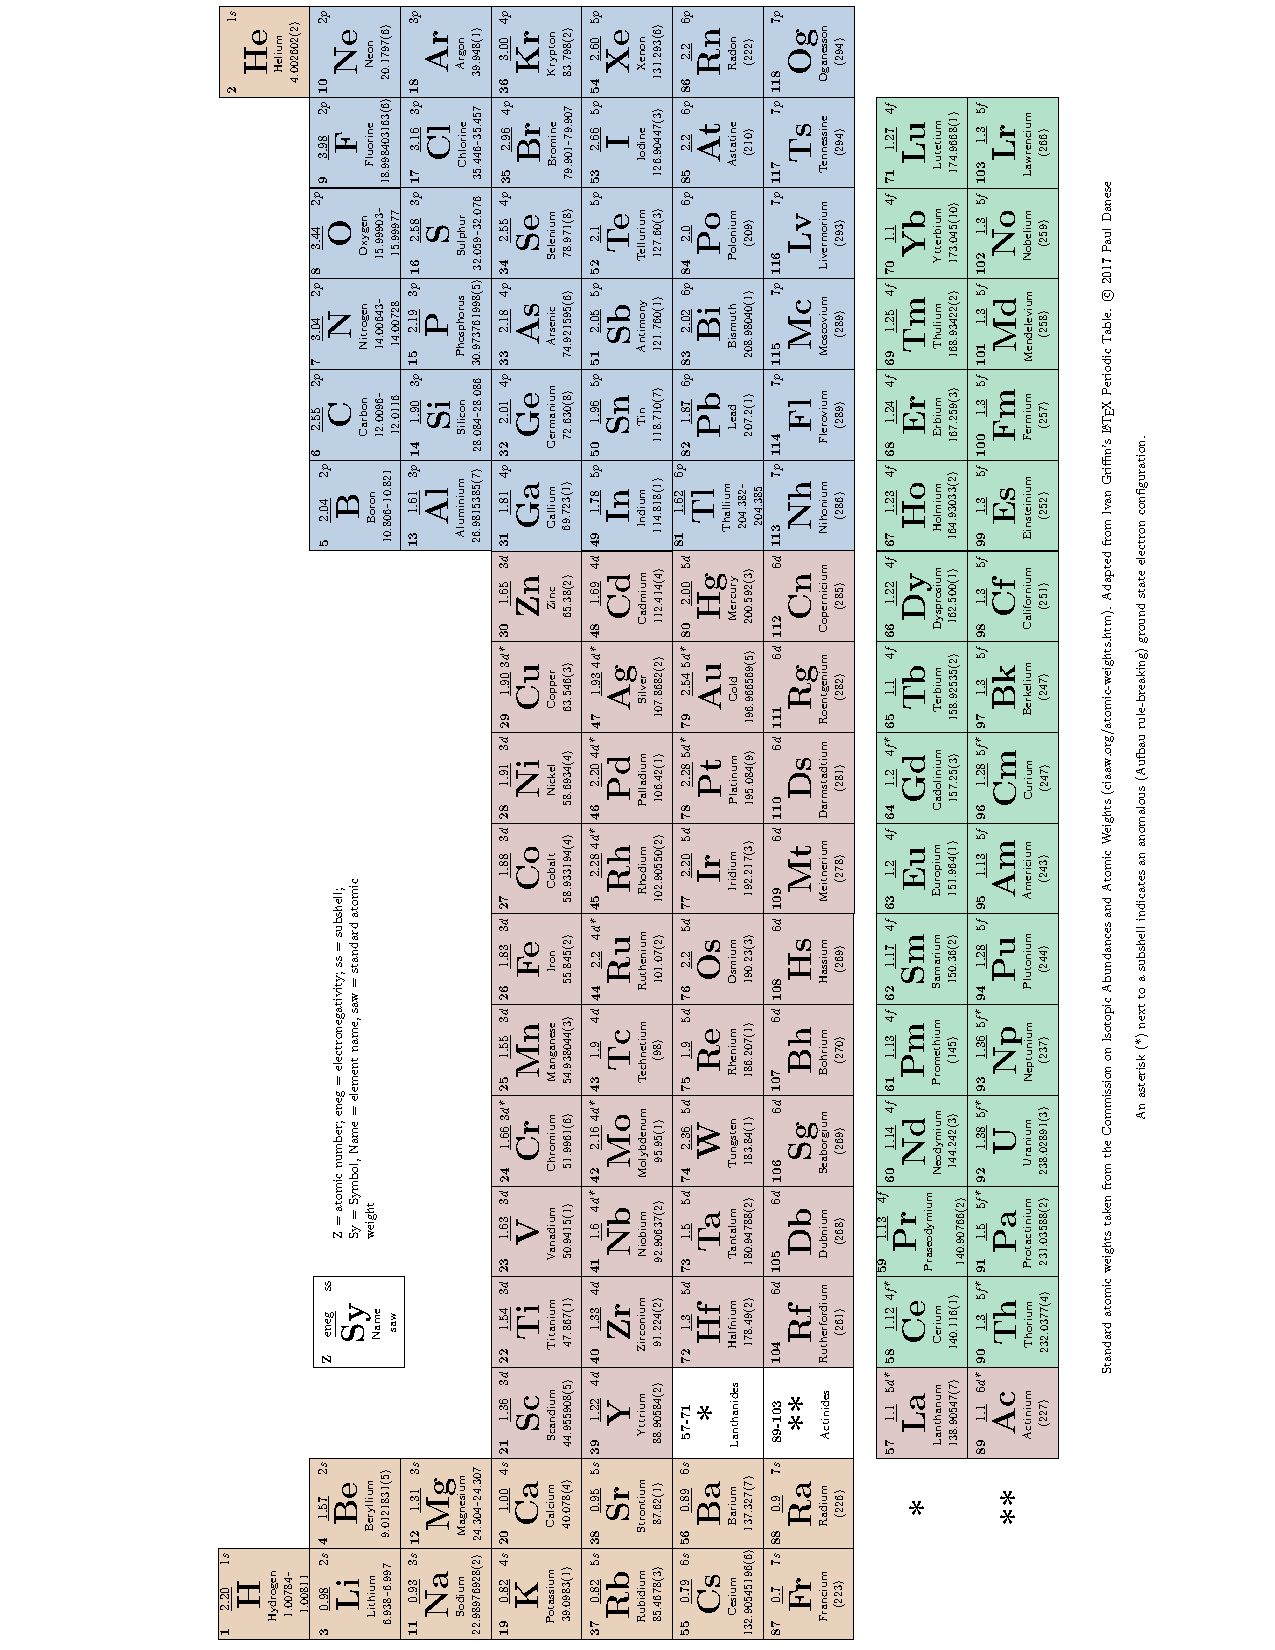
\includepdf[angle=-90,pagecommand={\section{Periodic Table of the Elements}}, scale=0.9]{periodic_table.pdf}

\end{document}
